%!TEX root = ../tesis.tex
\chapter{Desarrollo de la Ontología}
\label{chap:Desarrollo de la Ontologia}

Luego de haber estudiado las distintas metodologías para el desarrollo de ontologías, se decidió utilizar la metodología NeOn, ya que la misma según la tabla xx posee mayor especificación en las actividades a desarrollar  y contempla los caso de reuso de recursos ontológicos y no-ontológicos. 

Siguiendo la metodología NeOn se identifica que la ontología a desarrollar sigue las actividades compuestas principalmente por los escenarios 1, 2 y 3 que se exponen de la metodología. El escenario 1, puesto que se quiere modelar una ontología desde el principio y es la base de los demás escenarios, el escenario 2 y 3 ya que se pretende reusar recursos ontológicos y no-ontológicos. A continuación se detalla la primera actividad que consiste en la especificación de los requerimiento de la ontología.


\section{Especificación de requerimientos de la ontología}

En esta actividad se define el alcance y los requerimientos de la ontología a desarrollar. Como resultado de esta actividad se obtiene el Documento de Especificación de Requerimientos de la Ontología (ORSD). A continuación se detalla el resultado de dicho proceso.
\begin{enumerate}
\item \textbf{Propósito:} Crear una ontología para el dominio de Contrataciones Públicas para lograr la interoperabilidad semántica con otras fuentes de datos externas utilizando el OCDS como base de conocimiento principal aumentando la formalidad semántica como se muestra en la figura \ref{img:ocds-ocntology-complejidad}

\begin{figure}[h!]
\centering
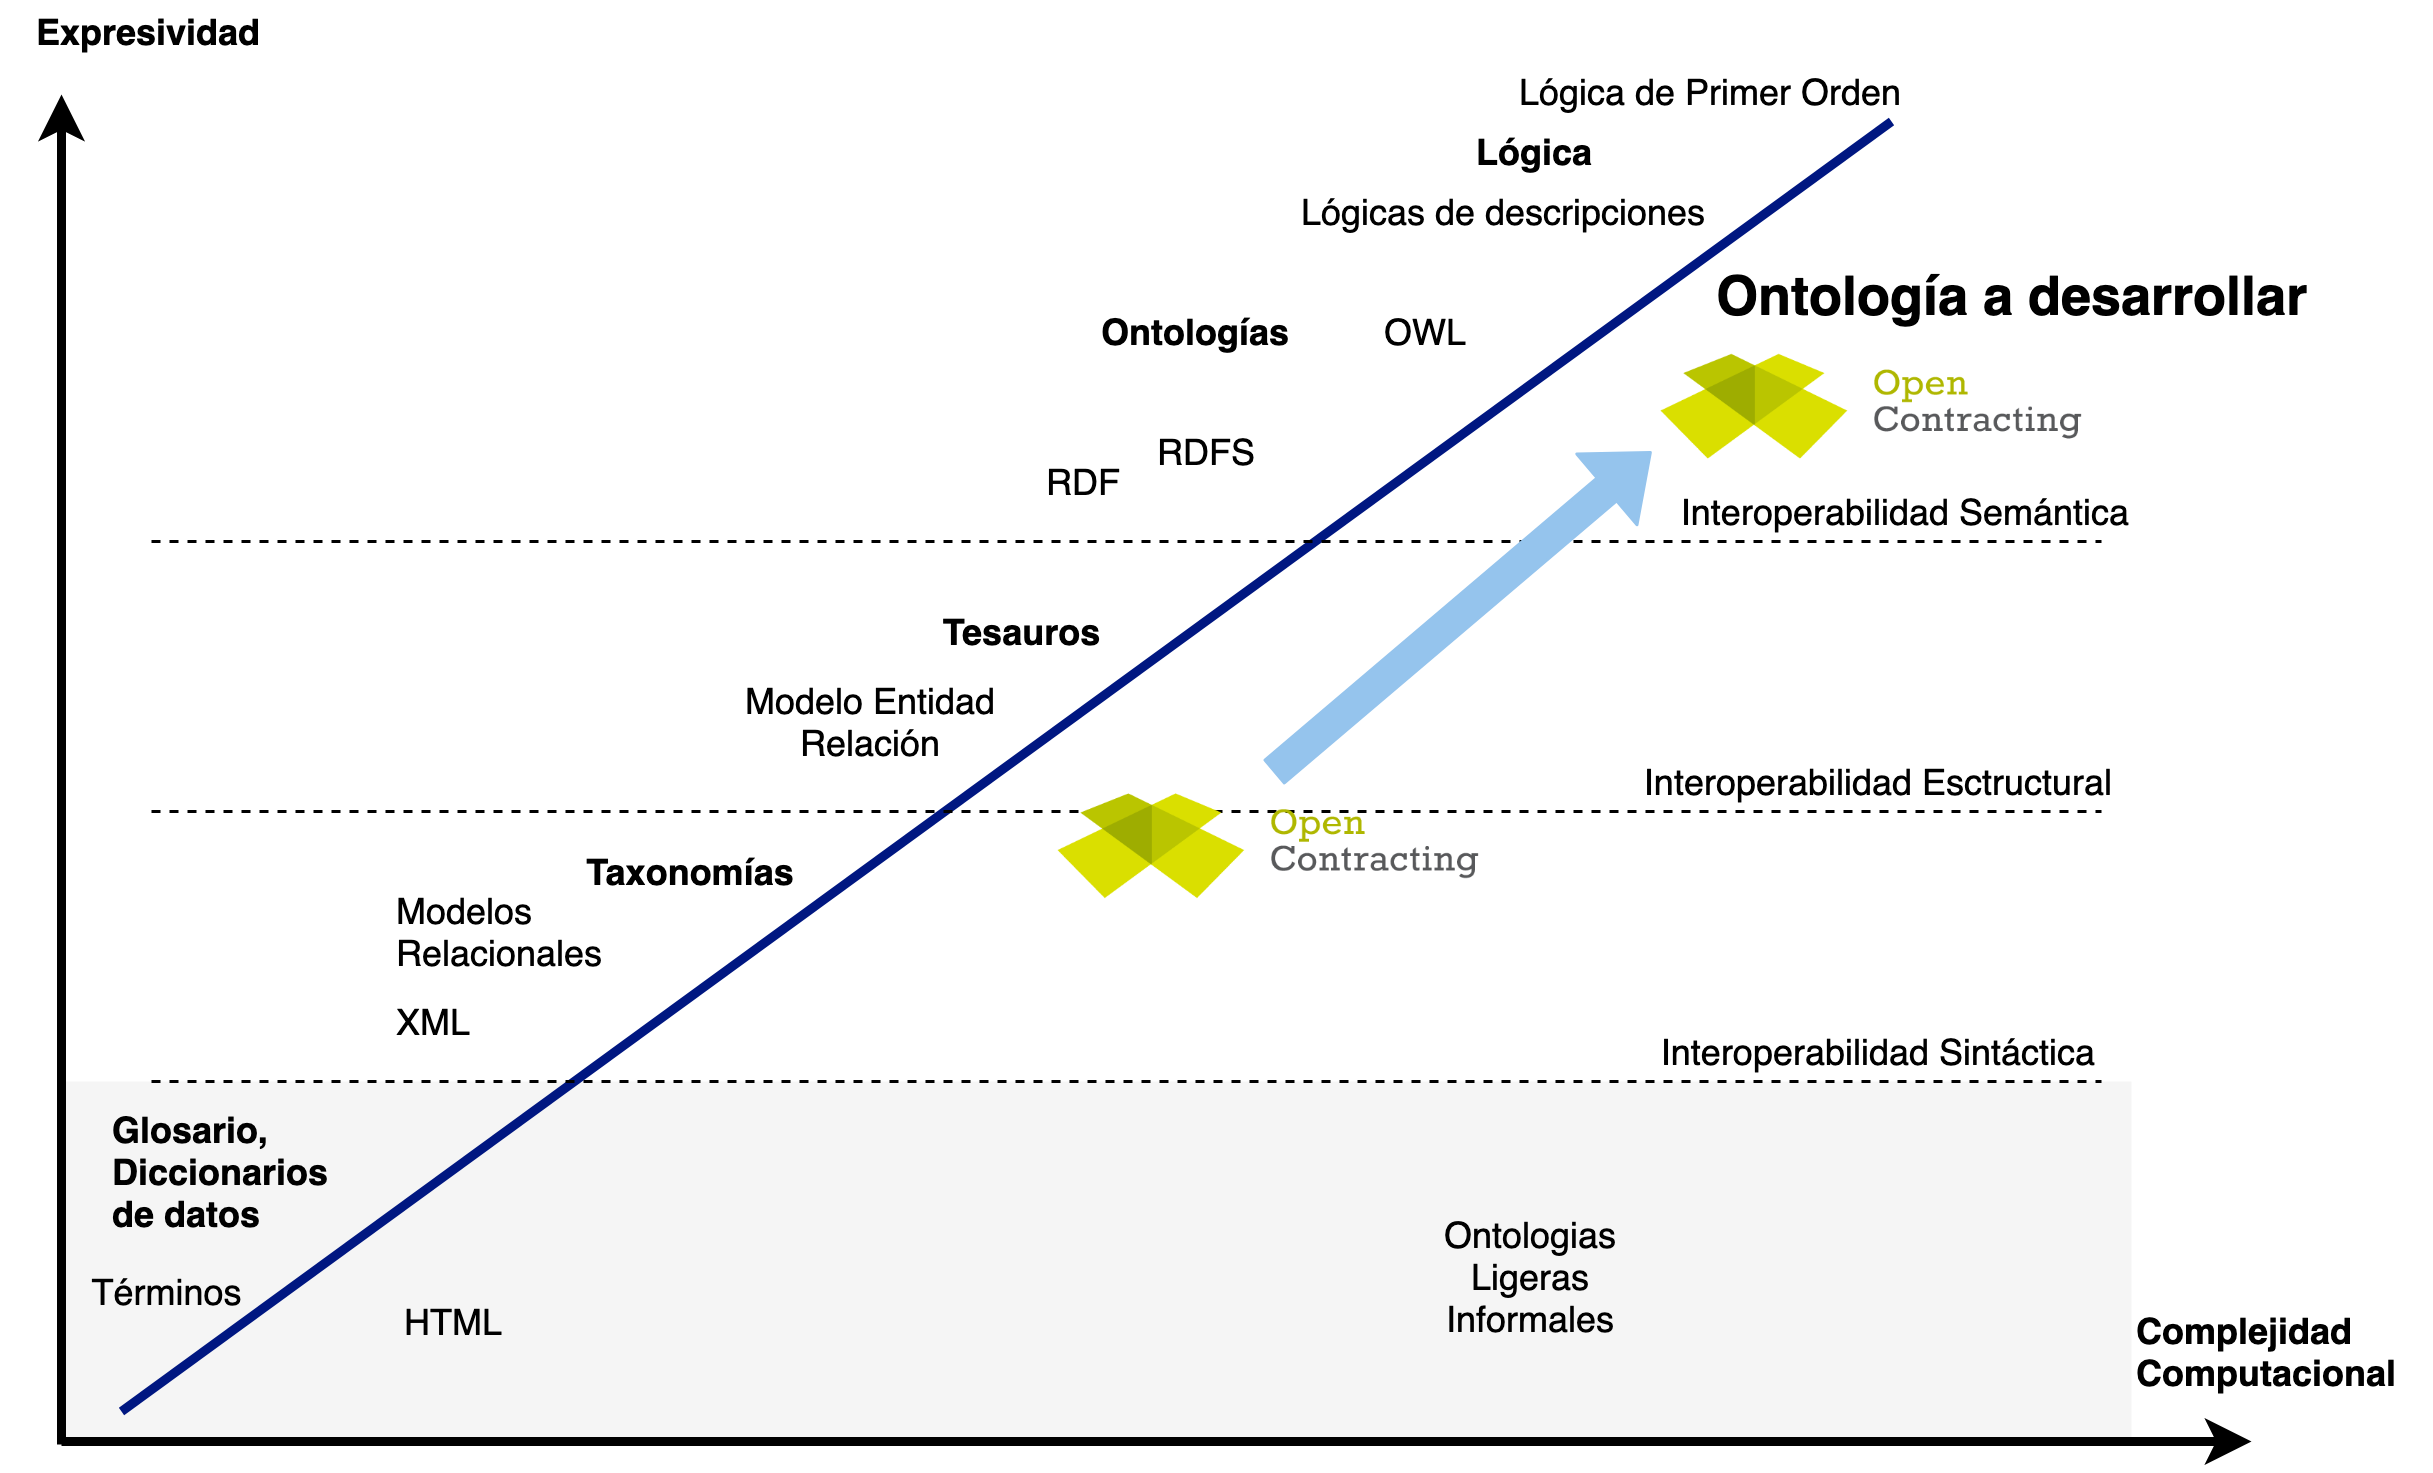
\includegraphics[width=150mm]{figuras/Diagramas-OenContracting.png}
\caption{Nivel de complejidad semántica de la ontología a desarrollar}
\label{img:ocds-ocntology-complejidad}
\end{figure}
\item \textbf{Alcance:} El alcance de la ontología está delimitada por el vocabulario detallado en la versión 1 del OCDS. Ya que en el momento del inicio de esta investigación era la última versión estable del estándar.
\item \textbf{Lenguaje de Implementación.} Se utilizará el lenguaje OWL debido a que es el lenguaje preferido para ontologías en la web semántica recomendado por la W3C, y se requiere de una ontología lo suficientemente ligera y explícita que se pueda manejar en la web semántica.
\item \textbf{Grupo Objetivo. }La ontología está orientada a:
\begin{enumerate}
    \item Expertos del dominio de Contrataciones Públicas que quieran realizar consultas ad-hoc sobre datos.
    \item Desarrolladores de software que deseen implementar el OCDS.
    \item Desarrolladores de software que necesiten integrar datos de contrataciones públicas con otras fuentes externas. \end{enumerate}
\item \textbf{Usos de la Ontología. }La ontología se utilizará para crear un esquema de publicación en JSON-LD, esto es debido a que la sintaxis JSON es ampliamente conocida y preferida por los desarrolladores, además el OCDS ya posee un esquema de publicación compatible con esta sintaxis. Los datos utilizados se extraerán del portal de datos abiertos de la DNCP.
\item \textbf{Requerimientos No Funcionales: }
\begin{enumerate}
    \item Se optará, en lo posible, por la reutilización de otras ontologías del dominio de Contrataciones Públicas ampliamente utilizadas.
    \item La ontología desarrollada debe ser procesable dentro de las limitaciones de la web semántica, ósea debe ser una ontología ligera.
    \item Debe soportar múltiples lenguajes: inglés y español inicialmente.
\end{enumerate}
\item \textbf{Requerimientos Funcionales. }
    \begin{enumerate}
        \item Gracias a la ontología se podrán responder las mismas preguntas que se responden a través de los datos publicados en formato de JSON y se podrán responder preguntas de todas las fases del proceso licitatorio.
        \item Debe ser compatible con la versión 1 del OCDS.
        \item Los datos deberán poder ser enriquecidos con otras fuentes de datos provenientes de la DNCP y también fuentes externas como Wikidata o DBpedia.
    \end{enumerate}
\item \textbf{Pre-Glosario de Términos.} El glosario fue extraído del diccionario de datos y de la ontología desarrollada por la DNCP. 
\end{enumerate}

\section{Planificación de las Actividades}

Linked Open Data se enfoca en un método de publicación de datos abiertos estructurados para que puedan ser interconectados. Para lograr esto se utilizan las tecnologías como RDF, RDFa, etc. para estructurar los datos, utilizando URIs para identificar los datos individualmente. Tim Berners Lee define un modelo de 5 estrellas para clasificar e identificar el grado de publicación de datos abiertos.

 


\section{Resumen}

